\documentclass[10pt, a4paper]{article}
\usepackage{ctex}   %For Chinese characters
\usepackage{amsmath, amsfonts, amssymb} %For equations
\usepackage{float}  %控制表格所在位置
\usepackage{enumerate}  %控制enumerate使用的符号
\usepackage{hyperref}   %超链接
\usepackage{graphicx}   %插入图像
% \usepackage{fullpage}   %直接设置页边距 只需要引入这个包就可以
\usepackage[top=1in, bottom=1in, left=0.5in, right=0.5in]{geometry} %自己设置页边距


\title{\LaTeX\ 测试}
\author{黄C}
\date{\today}

\parindent 0pt  %段落缩进
\pagestyle{empty}   %不显示页眉页脚
\begin{document}
\maketitle
\tableofcontents
Hello world!\LaTeX\

我

一个等式给出 $${f(x)=x^2 + 6x + 9}$$
$$2x^{35}$$
$$2x^{3x+4}$$
$$2x^{3x^{3x^4+5}+5}$$

子公式
$$x_1 + x_2 + ... + x_n = 3$$
$$a_1 + a_{1_{2_{3}}} = 18$$
$$x_1 + x_2 + \ldots + x_n = 3$$

特殊符号
$$\pi$$
$$\Pi$$
$$\alpha$$
$$A = \pi r^2$$
$$y=\csc \theta^2$$
$$y=\sin^{-1} x $$

$$y=\log x$$

$$\sqrt[2]{15}$$
$$\sqrt{2}$$
$$\sqrt{x^2+y^2}$$
$$\sqrt{1+\sqrt{x^2+y^2}}$$

分式
$$\frac{2}{3}$$
行内大写的方法$\displaystyle \frac{12}{80}$\\[8pt]
行内小写的方法$\frac{12}{80}$\\[8pt]
行内大写的方法$\dfrac{12}{80}$  %dfrac的使用需要用到包amssymb

$$\frac{\sqrt{1+x}}{\sqrt{1+y}}$$
$$\frac{1}{1+\frac{1}{x}}$$

括号
乘法结合律的简述$a(b+c)=ab+ac$,$\forall a, b, c \in \mathbb{R}$ \\
集合$A$是${1, 2, \ldots}$\\
价格$\$11.50$。

$2\left(\frac{1}{\sqrt{x^2+y^2}}\right)$
$2\left[\frac{1}{\sqrt{x^2+y^2}}\right]$
$2\left\{\frac{1}{\sqrt{x^2+y^2}}\right\}$
$2\left| \frac{1}{\sqrt{x^2+y^2}}\right| $

$$\left. \frac{dy}{dx}\right| _{(0, 1)}$$
$$\left( \frac{1}{1+\left(\frac{1}{1+x}\right)} \right) $$

表格:\\
\begin{table}[H]
    \centering  %表格居中
    \def\arraystretch{1.5}  %表格间隔
\begin{tabular}{|c||r|r|r|r|r|} %r右对齐 c中间对齐 l左对齐
    \hline
    $x$         & 1 & 2 & 3 & 4 & 5 \\    \hline
    $y$         & 1 & 2 & 3 & 4 & 5 \\    \hline
    $z$         & 1 & 2 & 3 & 4 & 5 \\    \hline
    $f(x, y, z)$ & $\frac{1}{10}$ & 20 & 30 & 40 & 50 \\  \hline
\end{tabular}
\caption{表格标题}
\end{table}

\begin{table}[H]
    \centering  %表格居中
    \def\arraystretch{1.5}  %表格间隔
\caption{还可以在这里}
\begin{tabular}{|c|p{5cm}|} %r右对齐 c中间对齐 l左对齐 p段落
    \hline
    $f(x)$ & $f'(x)$    \\  \hline
    $x > 0$ & The function $f(x)$ is increasing.The function $f(x)$ is increasing.
    The function $f(x)$ is increasing.The function $f(x)$ is increasing.
    The function $f(x)$ is increasing.The function $f(x)$ is increasing.  \\  \hline
\end{tabular}
\caption{表格标题}
\end{table}

Array:
\begin{align*}
    \text{这样才是文本,否则都是数学表达式。}   \\
    5x^2 + 10 &= 15\\
    &=12+x
\end{align*}

\begin{align}
    5x^2 + 10 &= 15\\   %加&表示等号对齐
    8x^3 + 12 &= 0
\end{align}

\vspace{1cm}

\begin{enumerate}
    \item 张三
    \item 李四
    \item 王五
    \item 逆天
        \begin{enumerate}
            \item 第一
            \item 第二
            \item 最后
                \begin{enumerate}
                    \item test
                    \item qulzzes
                \end{enumerate}
        \end{enumerate}
    \item 赵六
\end{enumerate}

\begin{enumerate}[A.]
    \item 123
    \item 456
    \item 79
\end{enumerate}

\begin{enumerate} \setcounter{enumi}{6}
    \item 123
    \item 456
    \item 79
\end{enumerate}

\vspace{1cm}

\begin{itemize}
    \item pencil
    \item ruler
    \begin{itemize}
        \item[(a)] notes
        \item[] homework
        \begin{itemize}
            \item test
        \end{itemize}
    \end{itemize}
\end{itemize}

斜体文字:\textit{这是斜体文字}。

加粗文字:\textbf{这是加粗文字}。

大写字母:\textsc{small caps}。

打字机体:\texttt{small caps}。
请访问 \texttt{https://www.youtube.com}

请访问 \href{https://www.youtube.com/watch?v=ydOTMQC7np0&t=6701s&ab_channel=freeCodeCamp.org}{原视频}

文字大写:这是测试文字

文字大写:\begin{large}这是测试文字\end{large}

文字大写:\begin{Large}这是测试文字\end{Large}

文字大写:\begin{LARGE}这是测试文字\end{LARGE}

文字大写:\begin{huge}这是测试文字\end{huge}

文字小写:\begin{small}这是测试文字\end{small}

文字小写:\begin{scriptsize}这是测试文字\end{scriptsize}

文字小写:\begin{tiny}这是测试文字\end{tiny}

\begin{center}文字位置:这是测试文字\end{center}

\begin{flushleft}文字位置:这是测试文字\end{flushleft}

\begin{flushright}文字位置:这是测试文字\end{flushright}

\section{第一章}
    \subsection{1.1}
        \subsection{1.1.1}
        \subsection{1.1.2}
    \subsection{1.2}
    \subsection{1.3}
\section{第二章}
    \subsection{2.1}
    \subsection{2.2}
    \subsection{2.3}

$$\forall x \in \mathbb{R}^2,\exists \varepsilon > 0,make\ x^2 \leqslant  \varepsilon $$
$$\forall x \in \mathbb{Z}^2,\exists \varepsilon > 0,make\ x^2 \leqslant  \varepsilon $$

\def\eq1{y=\dfrac{x}{3x^2+x+1}}

$$\eq1$$

\newcommand{\set}[1]{\setlength\itemsep{#1em}}
\begin{enumerate} \setcounter{enumi}{6}
    \set{0.5}
    \item 123
    \item 456
    \item 79
\end{enumerate}

\begin{center}
    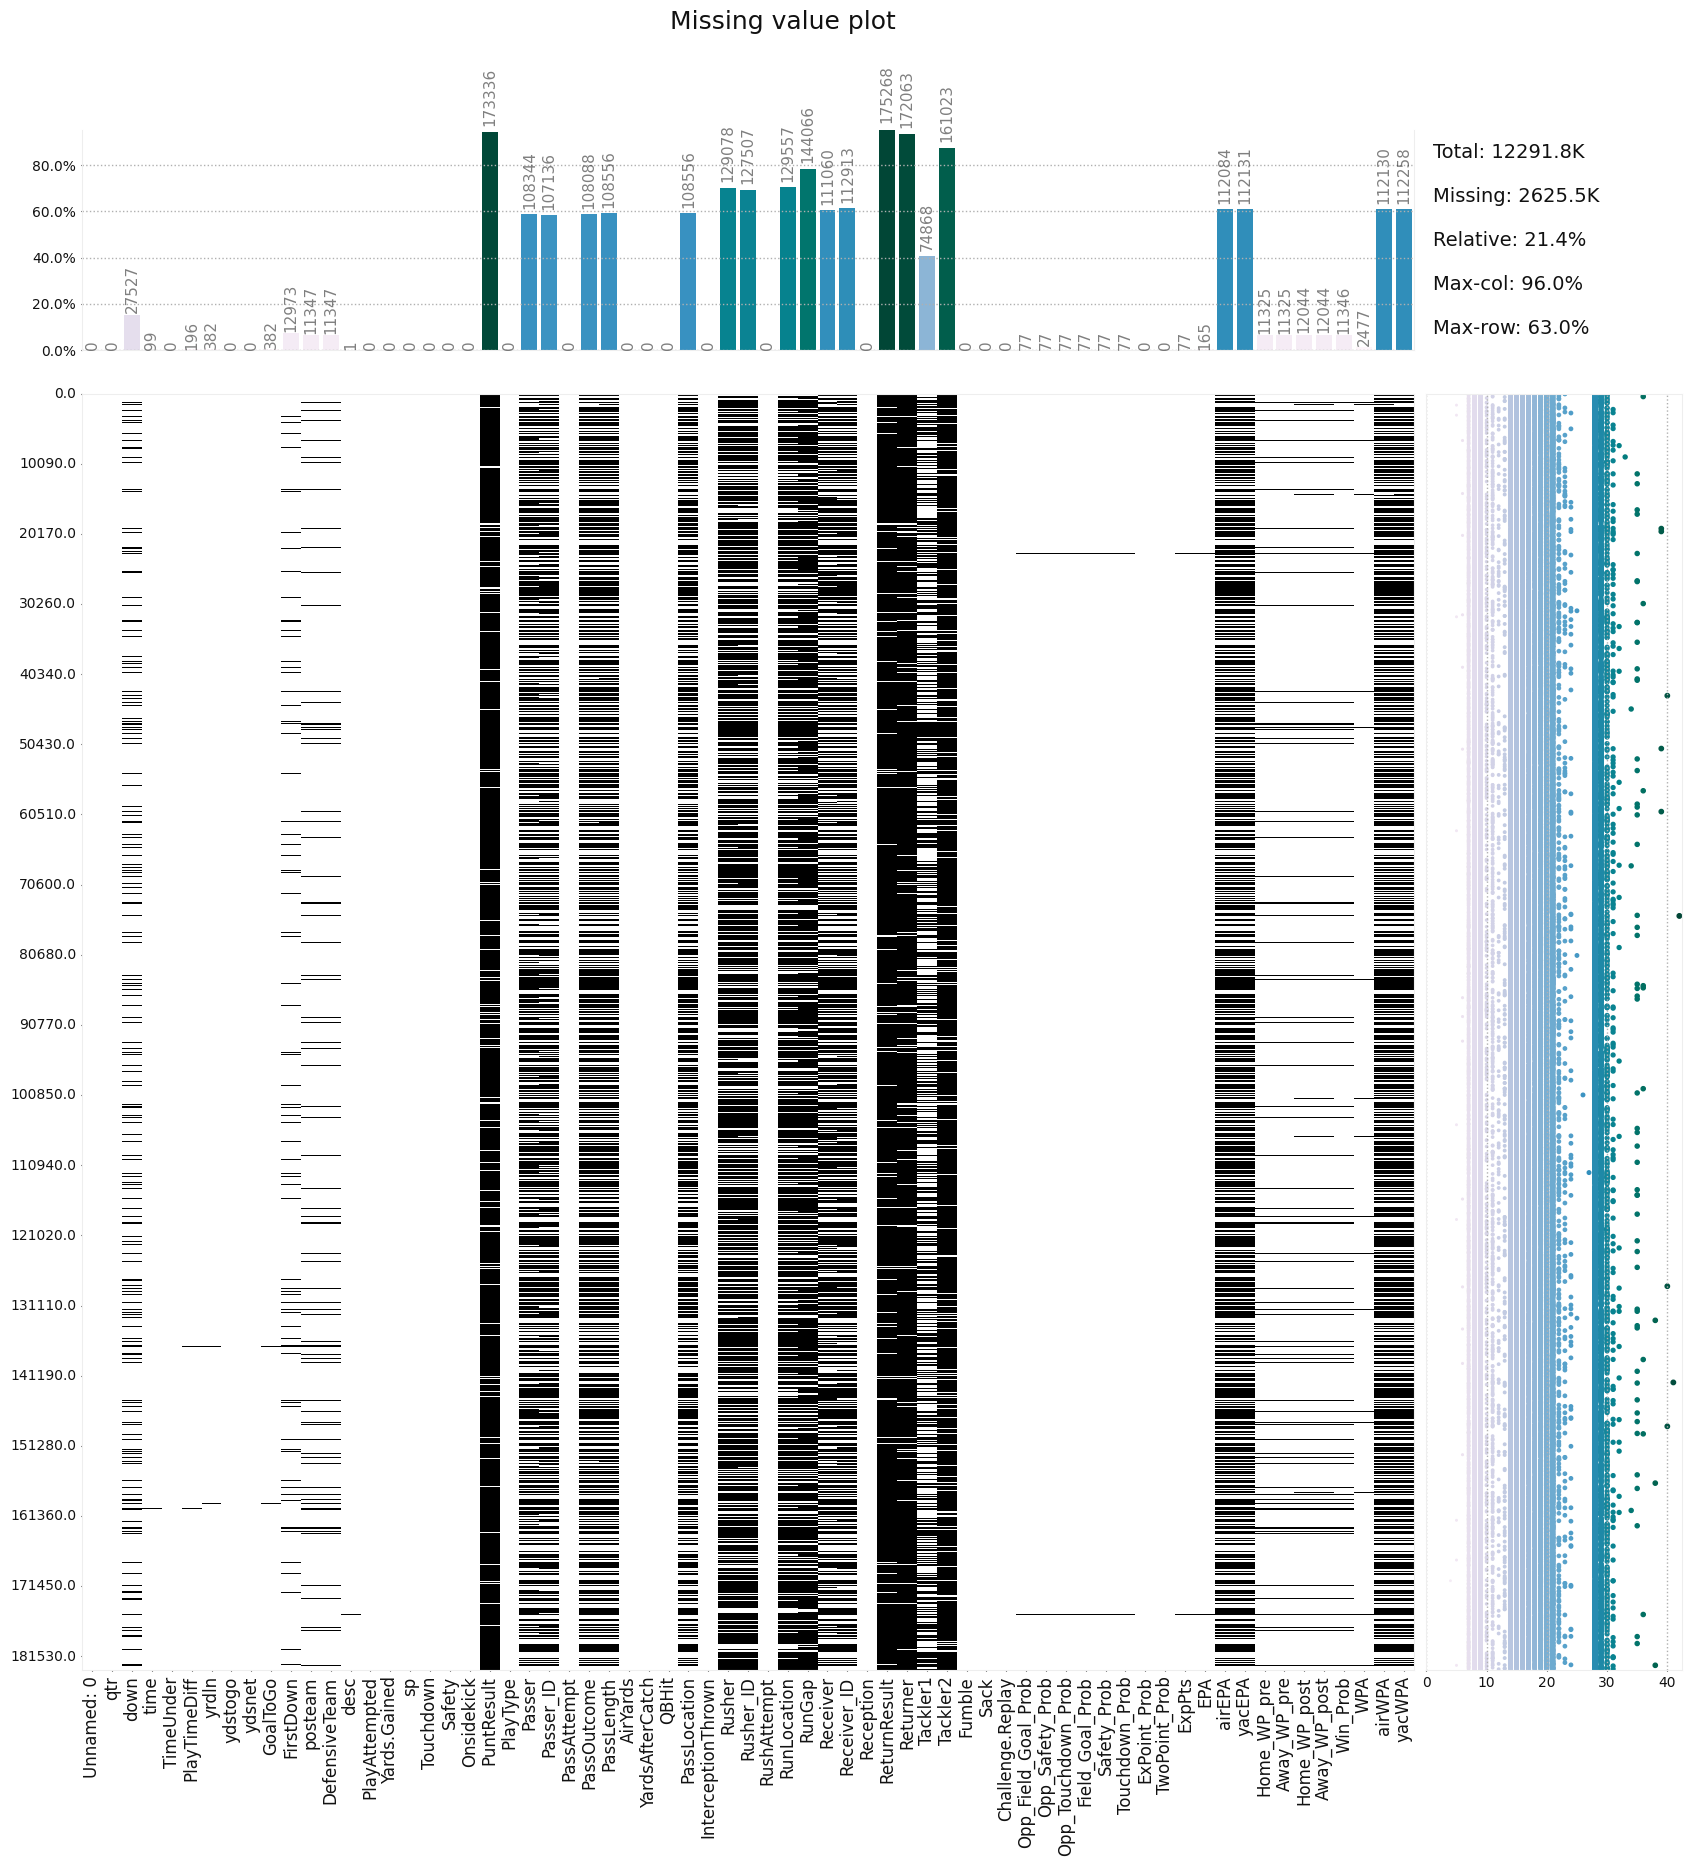
\includegraphics[width=0.4\textwidth]{output}
\end{center}

\begin{quote}
    \zihao{-5}\kaishu what can i say?啊
    \zihao{-5}\songti 还得是你
\end{quote}

\begin{abstract}
    这是一段小句子
\end{abstract}

\end{document} 
